%%%%%%%%%%%%%%%%%%%%%%%%%%%%%%%%%%%%%%%%%%%%%%%%%%%%%%%%%%%%%%%%%%%%%%
% Problem statement
\begin{statement}[
  problempoints=50,
  timelimit=1 second,
  memorylimit=512 MiB,
]{Pod starim krovovima}

\setlength\intextsep{-0.1cm}
\begin{wrapfigure}[7]{r}{0.16\textwidth}
\centering
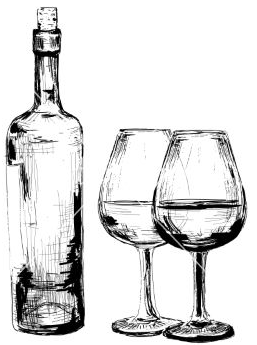
\includegraphics[width=0.16\textwidth]{img/psk.png}
\end{wrapfigure}

\textbf{Setting:} Legendary Zagrebian Inn called \textit{Kod Žnidaršića}.

\textbf{Time:} The year 1936.

\textbf{Plot summary:} Franjo and his friends are discussing the current events
in Abyssinia while enjoying a couple of drinks at the bar. His son, little
Perica, is sitting at a small table in the corner of the bar. In front of
Perica there are $N$ glasses conveniently numbered from $1$ to $N$. The volume
(in nanoliters) of each glass is known as well as the amount of liquid that
is currently inside it.

\textbf{Problem:} Little Perica wants to know what is the largest possible
number of glasses that can be emptied by pouring the liquid between glasses.
He can freely pour any integer number of nanoliters from one glass to another,
as many times as he wants, as long as no liquid is spilled over.

Your task is to output the number of empty glasses along with one possible
configuration of liquid in all glasses. If there are multiple configurations
that yield the same number of empty glasses, output any of them. Note that it
is not necessary to minimize the number of times liquid was poured between two
glasses.

%%%%%%%%%%%%%%%%%%%%%%%%%%%%%%%%%%%%%%%%%%%%%%%%%%%%%%%%%%%%%%%%%%%%%%
% Input
\subsection*{Input}
The first line contains an integer $N$ $(1 \le N \le 1\ 000)$ from the task
description.

Each of the next $N$ lines contains two integers $T_i$ $(0 \le T_i \le 10^9)$
and $Z_i$ $(1 \le Z_i \le 10^9)$ which, in that order, represent the current
amount of liquid in the $i$-th glass and its volume. Both quantities are
given in nanoliters and the current amount of liquid cannot be greater than
the volume of the glass, i.e.  $T_i \le Z_i$ holds.

%%%%%%%%%%%%%%%%%%%%%%%%%%%%%%%%%%%%%%%%%%%%%%%%%%%%%%%%%%%%%%%%%%%%%%
% Output
\subsection*{Output}
In the first line you should output the largest number of glasses that
can be emptied by pouring the liquid between glasses.

In the second line you should output the amount of liquid in each of the
glass after Perica has performed the necessary pourings. The glasses should
be ordered from glass numbered $1$ to glass numbered $N$.

%%%%%%%%%%%%%%%%%%%%%%%%%%%%%%%%%%%%%%%%%%%%%%%%%%%%%%%%%%%%%%%%%%%%%%
% Scoring
\subsection*{Scoring}
Correctly written first line is worth $4$ points, and correctly written second
line is worth $1$ point for each test case.

In test cases worth a total of $20$ points, all glasses will have the same
volume.

%%%%%%%%%%%%%%%%%%%%%%%%%%%%%%%%%%%%%%%%%%%%%%%%%%%%%%%%%%%%%%%%%%%%%%
% Examples
\subsection*{Examples}
\begin{tabularx}{\textwidth}{X'X'X}
\sampleinputs{test/psk.dummy.in.1}{test/psk.dummy.out.1} &
\sampleinputs{test/psk.dummy.in.2}{test/psk.dummy.out.2} &
\sampleinputs{test/psk.dummy.in.3}{test/psk.dummy.out.3}
\end{tabularx}

\textbf{Clarification of the second example:}
One of the possible pouring configurations is the following:
\begin{enumerate}
  \item pour everything from glass $1$ into glass $2$.
  \item pour everything from glass $2$ into glass $4$.
  \item pour four nanoliters from glass $3$ into glass $4$.
  \item pour one nanoliter from glass $3$ into glass $5$.
\end{enumerate}
Glasses numbered $1$, $2$ and $3$ are now empty.

%%%%%%%%%%%%%%%%%%%%%%%%%%%%%%%%%%%%%%%%%%%%%%%%%%%%%%%%%%%%%%%%%%%%%%
% We're done
\end{statement}

%%% Local Variables:
%%% mode: latex
%%% mode: flyspell
%%% ispell-local-dictionary: "croatian"
%%% TeX-master: "../hio.tex"
%%% End:
